The question of the existence of an analog to bound entanglement was firstly posed in \cite{GisWolf00} by Gisin and Wolf, where they analyzed the comparisons and correspondences between quantum and classical protocols for key agreement. 
The rise of bound information was a consequence of these correspondences.
Since then the topic was picked up by the scientific community of quantum cryptography and a couple more observation were made.
A probability distribution that presents bound information has not been found yet.
% Nevertheless 	a case for asymptotic bound information was proposed again by Wolf together with Renner \cite{RW03}.

\section{Tripartite bound information}
    A later work by Ac\'in et al. proposed the existence of bound information in a tripartite case \cite{ACM04}. 
    They analyzed the probability distribution resulting from measurement of a known bound entangled state. 
    Furthermore they also show that this distribution can be \textit{activated} the same way as in quantum entanglement.
    This result is different from what we want to achieve because the probability distribution is divided among parties Alice, Bob and Claire, with Eve being a fourth party in the distribution. 
    In fact, their result of bound information is valid only when considering \emph{pairs} of honest parties from the original distribution.
\section{The gap between the bounds can be arbitrarily large}
    To distinguish and analyze the case of bound information some information theoretical measures are needed. 
    We already saw the secret key rate (section \ref{seckeyrate}) and the intrinsic information (section \ref{intrininfo}) and we already presented the question of bound information in terms of such measures. 
    In \cite{RW03} a new measure of \emph{reduced intrinsic information} $\redintrinfo{X}{Y}{Z}$ is introduced as an upper bound on secret key rate, lower than just the normal intrinsic information.
    \begin{equation} \label{eq:reducedintrinfo}
    	\redintrinfo{X}{Y}{Z} := \inf_{P_{U|XYZ}} (\intrinfo{X}{Y}{ZU} + \Ent (U))
    \end{equation}
    For every $P_{XYZ}$ it holds
    \begin{equation} \label{eq:bounds}
    	\keyrate{X}{Y}{Z} \leq \redintrinfo{X}{Y}{Z} \leq \intrinfo{X}{Y}{Z}
    \end{equation}
    	Reduced intrinsic information is a strictly stronger upper bound on secret key rate than intrinsic information.
    	More importantly, Renner and Wolf proved that the gap between reduced and normal intrinsic information can be arbitrarily large. 
    	Considering then that the former is an upper bound to secret key rate, and the latter is a lower bound to information of formation, this implies then the existence of asymptotic bound information.
    	\begin{figure}[h!]
    		% scheme representing the bounds
% expresed in paper Renner+Wolf 2003
% on the quantities intrinsic information,
% secret key rate and information of formaion

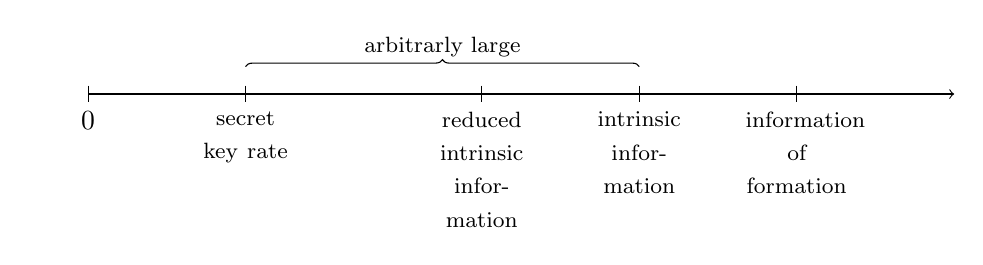
\begin{tikzpicture}
%	\tikzstyle{lineLabel}=[text width=10mm,align=center, below]
%	\draw[->] (0,0) -- (11,0);
%	\draw (0,.5) -- (0,-.5);
%	\draw (2,.5) -- (2,-.5);
%	\draw[dashed] (5,.5) -- (5,-.5);
%	\draw (7,.5) -- (7,-.5);
%	\draw (9,.5) -- (9,-.5);
%	
%	\node (zero) at (0,-.7) {$0$};
%	\node[lineLabel] (iof) at (9,-.7) {\footnotesize Information of formation};
%	\node[lineLabel] (inf) at (7,-.7) {\footnotesize Intrinsic Information};
%	\node[lineLabel] (rinf) at (5,-.7) {\footnotesize Reduced Intrinsic Information};
%	\node[lineLabel] (skr) at (2,-.7) {\footnotesize secret key rate};

\tikzset{
    position label/.style={
       below = 3pt,
       align=center,
%       text height = 1.5ex,
%       text depth = 1ex,
       text width=13mm
    },
   brace/.style={
     decoration={brace},
     decoration={raise=3ex},
     decorate
   },
   blabel/.style={
		above = 13pt,
		align=center,
		pos=0.5   
   }
}

% draw horizontal line
\draw[->] (0,0) -- (11,0);

%draw vertical lines
\foreach \x in {0,2,5,7,9}
   \draw (\x cm,3pt) -- (\x cm,-3pt);

%labels
\node [position label] (Start) at (0,0) {$0$};
\node [position label] (skr) at (2,0) {\footnotesize secret key rate};
\node [position label] (rinf) at (5,0) {\footnotesize reduced intrinsic information};
\node [position label] (inf) at (7,0) {\footnotesize intrinsic information};
\node [position label] (iof) at (9,0) {\footnotesize information of formation};

\draw [brace] (skr.north) -- node [blabel] {\footnotesize arbitrarly large} (inf.north);

\end{tikzpicture}
    		\caption{The different measures for $P_{XYZ}$ and how they bound each other.}
    	\end{figure}
    	
\section{A candidate probability distribution}\label{daproblem}
    Wolf and Renner proposed in \cite{RW03} for the first time a probability distribution (Fig. \ref{Tab:candidate}) which is a good candidate for the classical analogy of \emph{bound entanglement}. 
    In fact, they offer a probability distribution that asymptotically has bound information. 
    This example did not come directly from a translation of bound entangled states.
    They also show, for such a distribution, that 
    \begin{equation}
    	\keyrate{X}{Y}{Z} \neq \intrinfo{X}{Y}{Z}
    \end{equation}  
     and they emphasize that this is the first time that equality does not hold. This fact disproved the conjecture posed in \cite{MW99}, that the two measured were actually the same.
     
     For this probability distribution we have
	$$ \intrinfo{X}{Y}{Z} = 3/2 ,\; \keyrate{X}{Y}{Z} = 1 , \; \redintrinfo{X}{Y}{Z} = 1 $$
	With the the fact that $\redintrinfo{X}{Y}{Z} = \keyrate{X}{Y}{Z}$ does indeed happen, and with the statements above, we can think of a model to later search for bound information in chapter \ref{ch:six}. 
	If the reduced intrinsic information is a useful measure, we can minimize it to find probability distributions that have no possible key extractable from it.
     
	\begin{figure}
		%Table of probability distribution given in paper

	\begin{center}
		\begin{tabular}{|l r||c|c|c|c|}
		    \hline 
		    		 &	$X$ & $0$ & $1$ & $2$ & $3$ \\ 
		    $Y$ &		  &		&			&			&		\\
		    \hline 
		    \hline
		    $0$ &		   & $1/8$ & $1/8$ & $0$ & $0$ \\ 
		    \hline 
		    $1$ &		   & $1/8$ & $1/8$ & $0$ & $0$ \\ 
		    \hline 
		    $2$ &		   & $0$ & $0$ & $1/4$ & $0$ \\ 
		    \hline 
		    $3$ &		   & $0$ & $0$ & $0$ & $1/4$ \\ 
		    \hline 
		  \end{tabular} 
	\end{center}		

%\begin{table}[pos]
%\centering
%\caption{My caption}
%\label{my-label}
%\begin{tabular}{|l|l|l|l|l|l|}
%\hline
%\multicolumn{2}{|r|}{$X$} & \multirow{2}{*}{0} & \multirow{2}{*}{1} & \multirow{2}{*}{2} & \multirow{2}{*}{3} \\
%\multicolumn{2}{|l|}{Y}   &                    &                    &                    &                    \\ \hline
%\multicolumn{2}{|l|}{0}   & 1/8                & 1/8                & 0                  & 0                  \\ \hline
%\multicolumn{2}{|l|}{1}   & 1/8                & 1/8                & 0                  & 0                  \\ \hline
%\multicolumn{2}{|l|}{2}   & 0                  & 0                  & 1/4                & 0                  \\ \hline
%\multicolumn{2}{|l|}{3}   & 0                  & 0                  & 0                  & 1/4                \\ \hline
%\end{tabular}
%\end{table}
		
	    $$Z \equiv X + Y\; (mod\: 2)\; \text{ if } X,Y \in \{ 0,1\}$$ 
	    $$Z \equiv X\; (mod\: 2)\; \text{ if } X \in \{ 2,3\}$$ 
	    $$U \equiv \lfloor X/2 \rfloor $$
	    \caption{Probability distribution proposed by Renner, Wolf and Skripsky in \cite{RW03} for which it holds that $\keyrate{X}{Y}{Z} \neq \intrinfo{X}{Y}{Z}$}
	    \label{Tab:candidate}
	\end{figure}	 
	
	More promising is another probability they offer at the end (Fig. \ref{Tab:candidate2}) which is a slight modification of the first. 
	Here Renner and Wolf conjecture that it might be possible to achieve bound information by different values of $a$. 
	They also noted, however, that for $a$ too big the correlation between Alice and Bob is lost, loosing also the key cost value (or information of formation).
	
	
	\begin{figure}
		%Table of candidate distribution 1

		\begin{center}
		\begin{tabular}{|l r||c|c|c|c|}
		    \hline 
		    		 &	$X$ & $0$ & $1$ & $2$ & $3$ \\ 
		    $Y$ &		  &		&			&			&		\\
		    \hline 
		    \hline
		    $0$ &		   & $1/8$ & $1/8$ & $a$ & $a$ \\ 
		    \hline 
		    $1$ &		   & $1/8$ & $1/8$ & $a$ & $a$ \\ 
		    \hline 
		    $2$ &		   & $a$ & $a$ & $1/4$ & $0$ \\ 
		    \hline 
		    $3$ &		   & $a$ & $a$ & $0$ & $1/4$ \\ 
		    \hline 
		  \end{tabular} 
	\end{center}
	
	\begin{align*}
			Z \equiv&\: X + Y\; (mod\: 2)\; \text{ if } X,Y \in \{ 0,1\}\\
	    	Z \equiv&\: X\; (mod\: 2)\; \text{ if } X,Y \in \{ 2,3\}\\
	    	Z =&\: (X,Y) \text{ otherwise} 
	\end{align*}
	
%			$$Z \equiv X + Y\; (mod\: 2)\; \text{ if } X,Y \in \{ 0,1\}$$ 
%	    	$$Z \equiv X\; (mod\: 2)\; \text{ if } X,Y \in \{ 2,3\}$$ 
%	    	$$Z = (X,Y) \text{ otherwise} $$
	    	
	    	\caption{A candidate probability distribution for bound information, for $a\geq 0$ (and renormalized).}
	    	\label{Tab:candidate2}
	\end{figure}
    